\documentclass[a4paper,11pt]{article}

\usepackage{aas_macros}

\usepackage[utf8]{inputenc}	
\usepackage[T1]{fontenc}
\usepackage{lmodern}
\usepackage{times}
\usepackage[margin=2cm]{geometry}
\usepackage{amsmath}
\usepackage{mathtools}
\usepackage{graphicx}
\usepackage{multirow}
\usepackage{blindtext}
\usepackage{hyperref}
\usepackage{float}

\usepackage{pgfplotstable} 
\usepackage{booktabs}
% \pgfplotsset{compat=1.18}


\graphicspath{ {./images/} }

\usepackage[czech]{babel}
\usepackage{graphicx}
\usepackage{amsmath}
\usepackage{xspace}
\usepackage{url}
\usepackage{indentfirst}
\usepackage{subcaption}
\usepackage{caption}
\usepackage{tabularx}
\usepackage{rotating}
\usepackage{tikz}
\usepackage[labelformat=parens,labelsep=quad,skip=3pt]{caption}

\usepackage{color}  
\usepackage{listings}

\definecolor{codegreen}{rgb}{0,0.6,0}
\definecolor{codegray}{rgb}{0.5,0.5,0.5}
\definecolor{codepurple}{rgb}{0.58,0,0.82}
\definecolor{backcolour}{rgb}{0.95,0.95,0.92}

\lstdefinestyle{mystyle}{
    backgroundcolor=\color{backcolour},   
    commentstyle=\color{codegreen},
    keywordstyle=\color{magenta},
    numberstyle=\tiny\color{codegray},
    stringstyle=\color{codepurple},
    basicstyle=\ttfamily\footnotesize\centering,        
    breaklines=true,                 
    captionpos=b,                                  
    numbers=left,                    
    numbersep=5pt,                  
    showspaces=false,              
    showstringspaces=false,
    showtabs=false,                  
    tabsize=2
}

\lstset{style=mystyle}


\widowpenalty 10000 \clubpenalty 10000 \displaywidowpenalty 10000
\setcounter{topnumber}{3}	  
\setcounter{bottomnumber}{3}	 
\setcounter{totalnumber}{6}	  
\renewcommand\topfraction{0.9}	 
\renewcommand\bottomfraction{0.9} 
\renewcommand\textfraction{0.1}	  
\intextsep=8mm \textfloatsep=8mm 

\renewcommand{\thesection}{\arabic{section}.}
\renewcommand{\thesubsection}{\thesection\arabic{subsection}.}
\makeatletter \def\@seccntformat#1{\csname the#1\endcsname\hspace{1ex}} \makeatother


\begin{document}

\noindent\hrulefill 
\begin{center}
\bigskip
\huge Profil jádra komety C/2023 A3 (Tsuchinshan-ATLAS)
\vspace{0.2cm}
\par \large F4191: Praktikum z astronomie 2
\par \large Artem Gorodilov
\vspace{0.2cm}
\par \large 26. ~listopadu 2024
\bigskip
\end{center}
\noindent\hrulefill 
\bigskip

\vskip10pt
    \begin{minipage}[t]{0.5\textwidth} 
        \section{Abstrakt}    
            V tomto článku jsem analyzoval snímek komety C/2023 A3 (Tsuchinshan–ATLAS). k datu 16.10.2024 19:31 (UT). Pozorování bylo provedeno na Letiště TŘI SUDY Kotvrdovice E 49°21'52'':N 016°47'14'' E ve filtru V, expoziční doba 16 s.
            \par Výpočty byly provedeny pomocí skriptu v Pythonu\textsuperscript{\cite{github}}.

        \section{Úvod} 
            Při dopadu slunečního větru na jádro komety dochází k úniku hmoty z jádra komety. Tento proces popisuje rovnice kontinuity, která říká, že hustota hmoty N(x) s rychlostí $\upsilon$ ve vzdálenosti x$^2$ od jádra komety.
            \begin{equation}
                N(x) \upsilon x^2 = const
            \end{equation}
            \par Tvrdí tedy, že hustota hmoty musí být nepřímo úměrná čtverci vzdálenosti od jádra komety. N(x) $\propto$  x$^{-2}$.
            \par Je důležité objasnit, že tato rovnice platí, pokud předpokládáme, že kometární jádro je bodovým zdrojem emise hmoty. 
            \par Radiální profil jasnosti opticky husté komety je dán rovnicí:
            \begin{equation}
                B(p) = K_1 \int N dl
            \end{equation}
            kde K$_1$ je konstanta, N je hustota hmoty a dl je delka elementu směrem pohledu. p = (x$^2$ - l$^2$)$^{1/2}$/$\Delta$, kde $\Delta$ je geocentrická vzdálenost komety.
            \par Dosadíme-li rovnici (1) do rovnice (2), dostaneme: 
            \begin{equation}
                B(p) = \frac{K_2}{p}
            \end{equation}
            kde K$_2$ je konstanta.
            \par Jako míru radiálního jasu povrchu použijeme logaritmickou derivaci \textsuperscript{\cite{1987ApJ...317..992J}}
            \begin{equation}
                m = \frac{d \ln B(p)}{d \ln p}
            \end{equation} 
            Pro jednoduchou kometu ve stabilním stavu by se tento parametr měl rovnat m = -1.
    \end{minipage}
    \hspace{10pt}
    \begin{minipage}[t]{0.5\textwidth} 
        \section{Zpracování dat} 
            Skript přijímá jako vstup obrázek .fits. Poté je třeba definovat oblast pozadí, načež skript určí průměrné počet counts v této oblasti a odečte je od obrázku. Průměrná hodnota pozadí a směrodatná odchylka: 
            \begin{center}
                C$_{bkg}$ = 1335 counts, $\sigma_{bkg}$ = 258 counts.
            \end{center}
            \par Skript pak určí střed jádra komety jako nejjasnější pixel (nejvíce detekovaných fotonů) v dané oblasti snímku.
            \begin{center}
                x$_{center}$ = 3819 px, y$_{center}$ = 973 px.
            \end{center}
            \par Pro převod px na arcsec jsem použil skript \texttt{barnard.py} z předchozí úlohy. Rozlišení obrazu máme:
            \begin{center}
                R = 11.1(6) arcsec/px.
            \end{center}
            Vybrané hvězdy pro kolibraci a rovníkové souřadnice jsou uvedeny na obrázku (\ref{fig:barnard_radec}) a (\ref{fig:barnard_sky}).

            \begin{figure}[H]
                \centering
                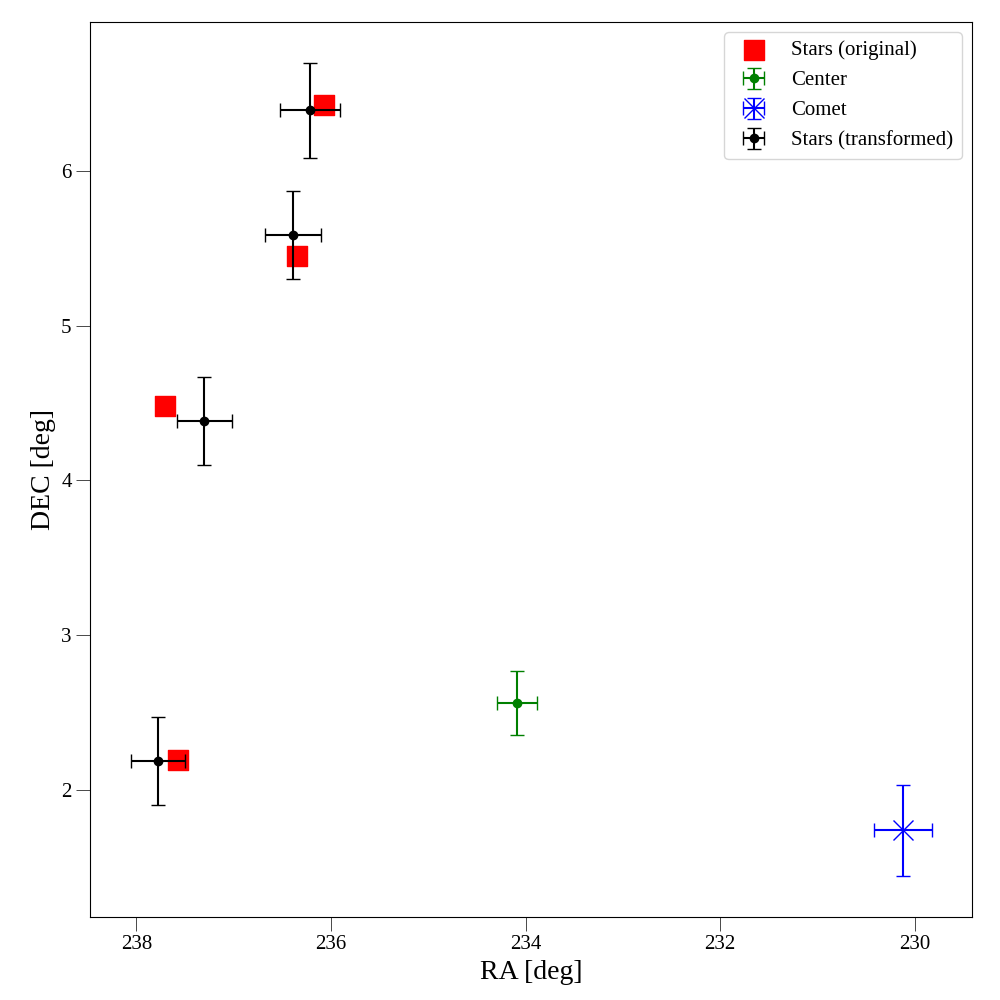
\includegraphics[scale=0.35]{barnard_radec}
                \captionsetup{justification=centering, font=footnotesize}
                \caption{Ekvatoriální souřadnice hvězd a komety}
                \label{fig:barnard_radec}
            \end{figure}
    \end{minipage}
\newpage
            \begin{figure}[H]
                \centering
                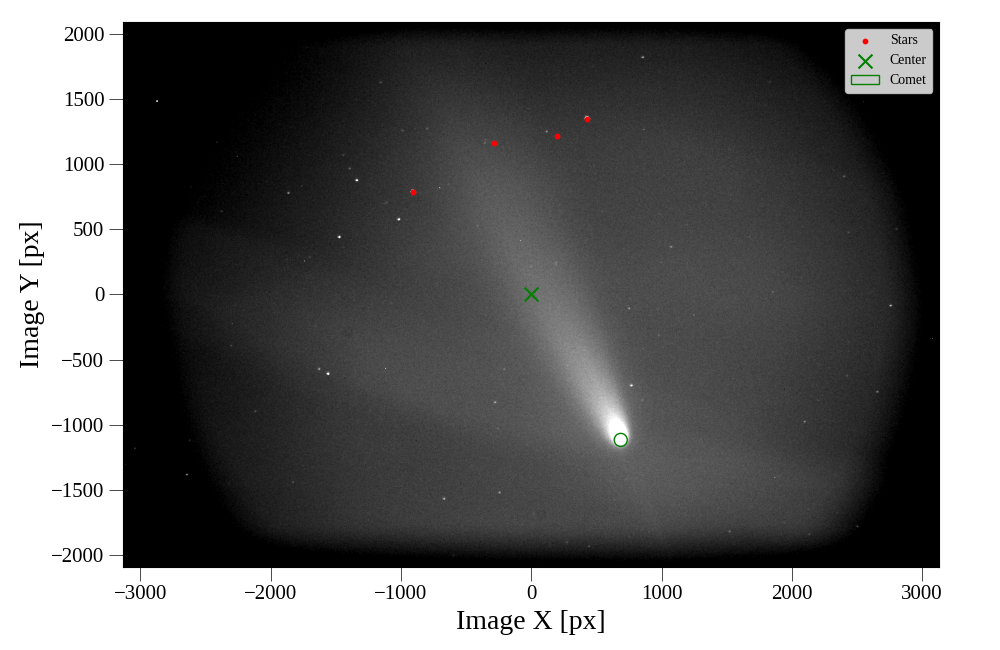
\includegraphics[scale=0.6]{barnard_sky}
                \captionsetup{justification=centering, font=footnotesize}
                \caption{Snímek noční oblohy s vyznačenými hvězdami, cometou a centrem čipu}
                \label{fig:barnard_sky}
            \end{figure}

    \begin{minipage}[t]{0.5\textwidth} 
            Dále je třeba určit jasnost komety v závislosti na vzdálenosti od jejího jádra. Obecně lze jako ukazatel jasnosti použít počet fotonů, které byly zachyceny na pixelu detektoru během doby expozice. Je také možné přepočítat počet countů $C$ na flux:
            \begin{equation}
                F = \frac{C}{t_{exp} S_{annulus}}
            \end{equation}
            \par a při znalosti zdánlivých hvězdných velikostí hvězd na snímku určit zdánlivou hvězdnou velikost oblasti komety:
            \begin{equation}
                m = m_{ref} - 2.5 \log_{10} \left( \frac{F}{F_{ref}} \right)
            \end{equation}
            \par Obě metody jsem vyzkoušel. 
            \par Ve svém obecném principu jsou založeny na následující myšlence: počítat počet countů z oblasti obrazu ohraničené dvěma prstenci. Střed prstenců bude ve středu jádra komety. Poloměry se zvětší na maximálně 50 px (vnější prstenec). Tím jsem vymezil oblast komety, která nás zajímá. Tuto oblast můžete vidět na obrázku (\ref{fig:comet_clean}).
            \par Výpočet jasu v countech je poměrně jednoduchý. Stačí sečíst všechny countů z oblasti ohraničené prstenci. Získání magnitudy je o něco složitější. Na snímku jsem našel 3 hvězdy, u kterých byly z literatury známy hodnoty zdánlivé hvězdné velikosti ve filtru V. Vybrané hvězdy jsou zobrazeny na obrázku (\ref{fig:comet}). Jejich magnitudy jsou následující: 
            \begin{center}
                m$_{modra}$ = 5.2, m$_{cervena}$ = 3.7, m$_{zelena}$ = 2.6.
            \end{center}
    \end{minipage}
    \hspace{10pt}
    \begin{minipage}[t]{0.5\textwidth}
            \vspace{-30pt}   
            \begin{figure}[H]
                \centering
                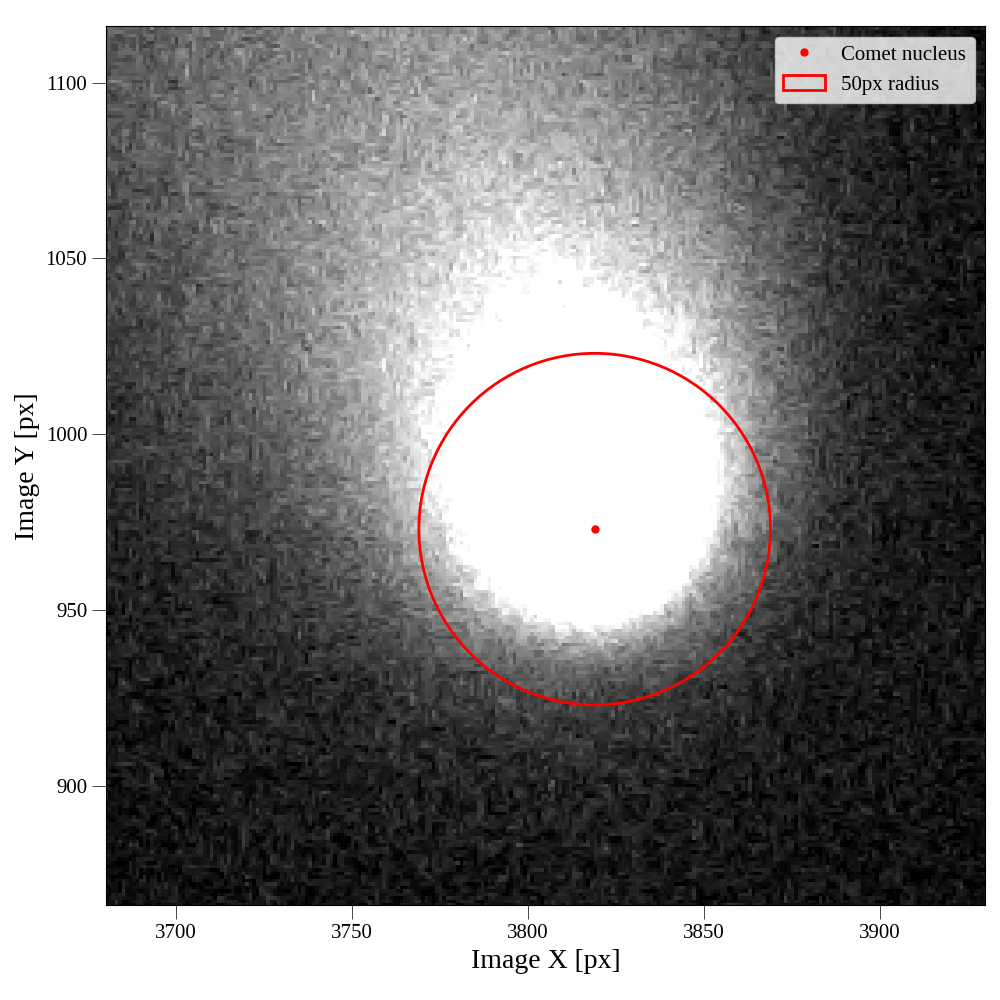
\includegraphics[scale=0.35]{comet_clean}
                \captionsetup{justification=centering, font=footnotesize}
                \caption{Obrázek komety s vyznačenou oblastí zájmu}
                \label{fig:comet_clean}
            \end{figure}

        \section{Vysledky}
            Jako první výsledek jsem získal zdánlivou hvězdnou velikost jádra komety: 
            \begin{center}
                m$_V$ = 2.1(9)
            \end{center}
            \par pro srovnání, v den pozorování Stellarium uvádí, že kometa měla hvězdnou velikost m = 1.05 mag.
        
    \end{minipage}
\newpage
            \begin{figure}[H]
                \centering
                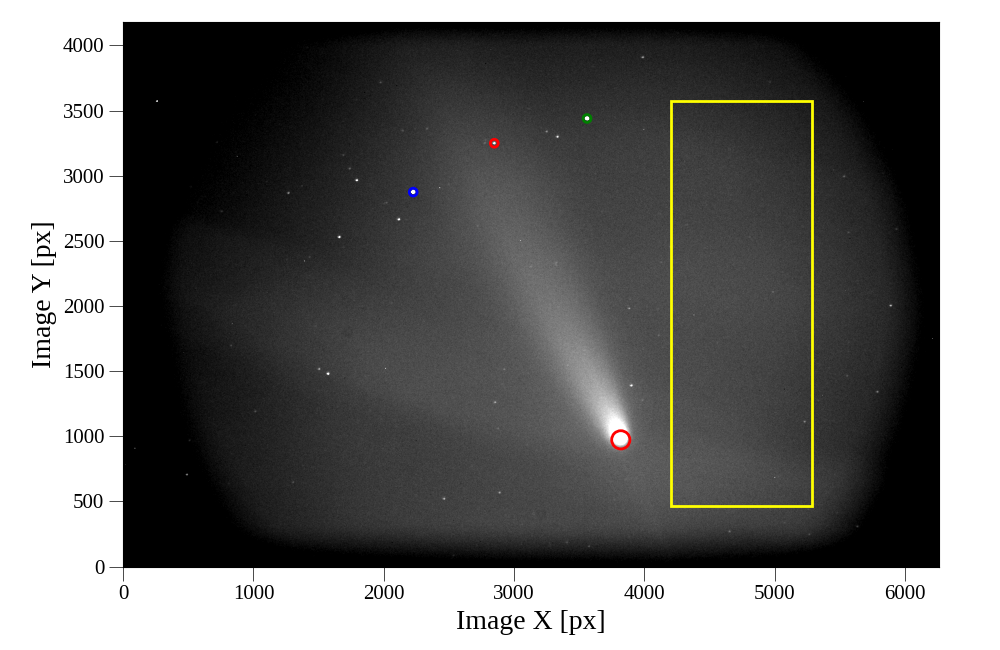
\includegraphics[scale=0.6]{comet.png}
                \captionsetup{justification=centering, font=footnotesize}
                \caption{Obrázek komety s kalibračními hvězdami a oblastí pozadí}
                \label{fig:comet}
            \end{figure}
            Poté jsem získal grafy profilu jasu povrchu (dále jen SBP). Pro lineární aproximaci jsem vybral oblasti nacházející se ve vzdálenosti log(p) > 1.75 arcsec. Pro obě metody byly získány následující hodnoty m:
            \begin{center}
                m$_{mag}$ = -3.3(2), m$_{counts}$ = -1.12(7)
            \end{center}
            Grafy SBP a gradientů m pro obě metody jsou znázorněny na obrázkách (\ref{fig:all_plots}).

        \section{Závěr}
            Jak je vidět, pro různé metody získávání SBP dostáváme různé hodnoty m. Bohužel se mi nepodařilo najít spolehlivé údaje o hodnotě m pro kometu C/2023 A3, abych je mohl porovnat s mnou získanými hodnotami. 
            \par Nejblíže „očekávanému“ teoretickému výsledku je metoda, při které jsme jako míru jasnosti vzali countů m = -1.12(7) s ideálním m = -1. Důvodem odchylky získané hodnoty od teoretické může být výrazná změna profilu komety v důsledku působení slunečního větru na její jádro. Jak je vidět na obrázku (\ref{fig:comet_clean}), hmota vyvržená z jádra je zřetelně protažena ve směru osy Y. 
            \par Pokud jde o výsledek získaný metodou magnitudy, podle mého názoru jsme takovou hodnotu mohli získat kvůli šumu na snímku. Přesněji řečeno, počasí bylo poměrně zamračené, výška komety nad obzorem nebyla příliš vysoká a kalibrační hvězdy byly relativně vyšší. Seeing tak způsobil vážné změny v přesnosti měření a pravděpodobně nemohl umožnit adekvátní výpočet prstencových magnitud. 
            
    \bibliographystyle{plain}
    \nocite{*}
    \bibliography{refs/github, refs/jewitt}

\newpage
    \begin{figure}[htbp]
        \centering
        \begin{subfigure}[t]{0.48\textwidth}
            \centering
            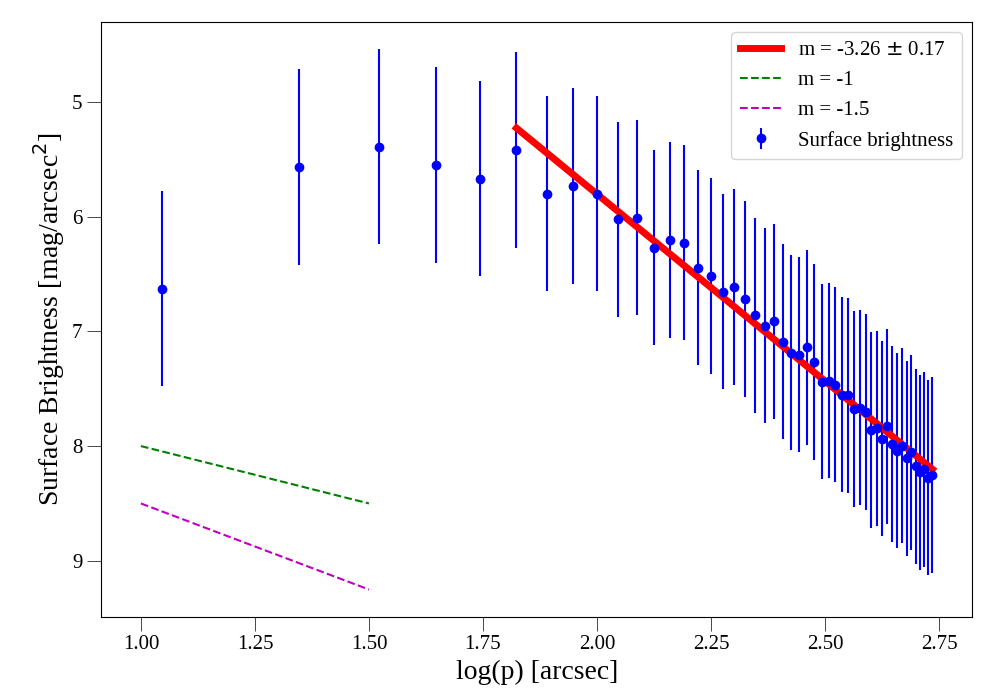
\includegraphics[width=\textwidth]{sbp.png}
            \captionsetup{justification=centering, font=footnotesize}
            \caption{Radiální profil jasu povrchu komety (mag)}
            \label{fig:sbp}
        \end{subfigure}
        \hfill 
        \begin{subfigure}[t]{0.48\textwidth}
            \centering
            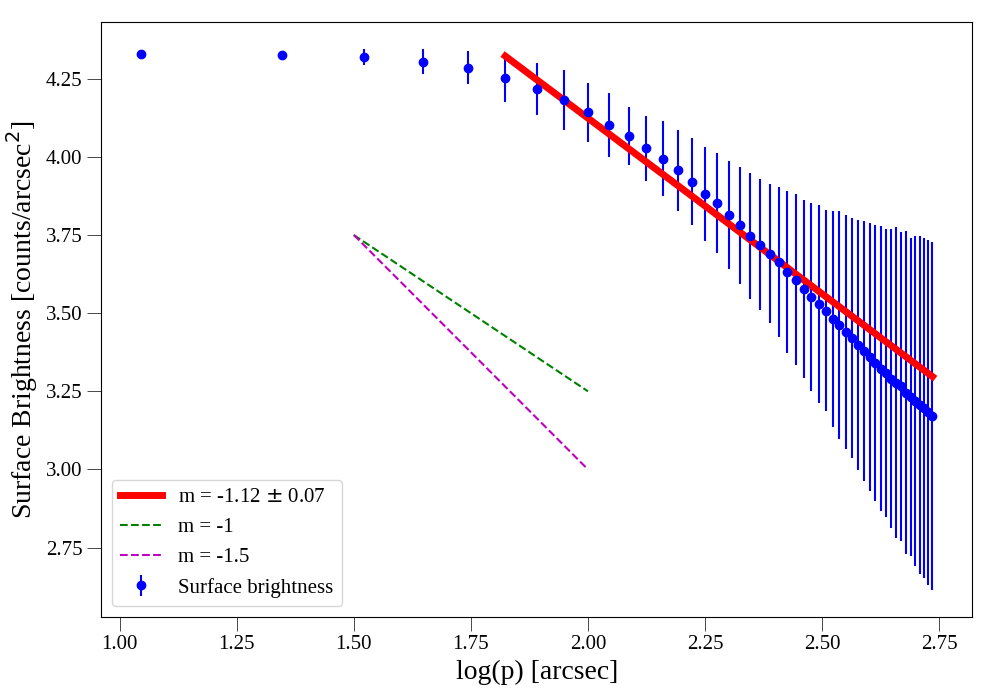
\includegraphics[width=\textwidth]{sbp_counts.png}
            \captionsetup{justification=centering, font=footnotesize}
            \caption{Radiální profil jasu povrchu komety (counts)}
            \label{fig:sbp_counts}
        \end{subfigure}
        \vspace{10pt} 
        \begin{subfigure}[t]{0.48\textwidth}
            \centering
            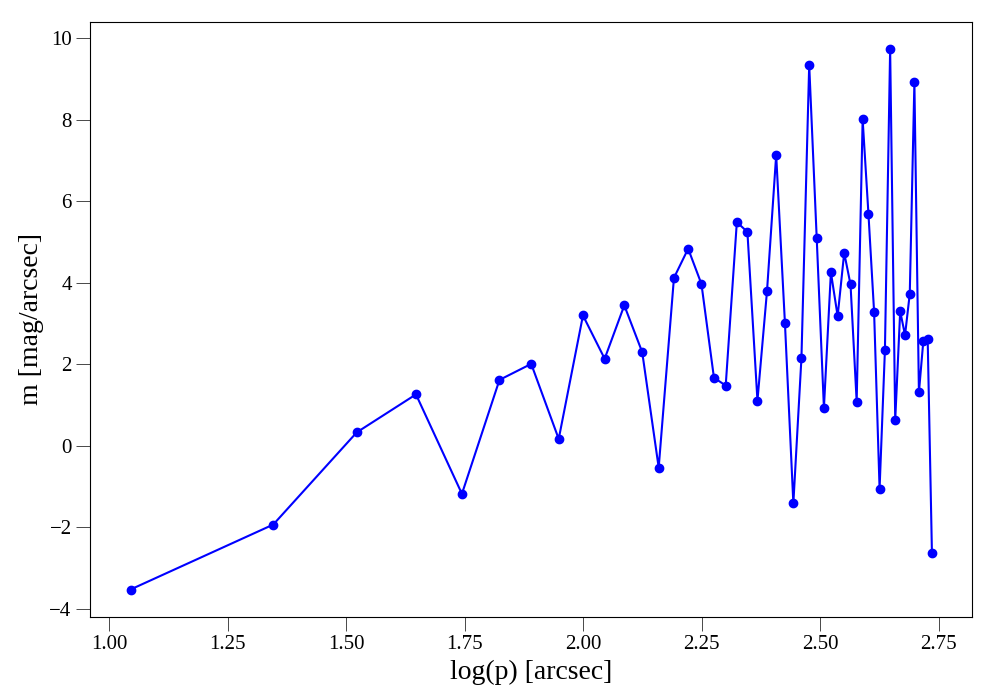
\includegraphics[width=\textwidth]{grad.png}
            \captionsetup{justification=centering, font=footnotesize}
            \caption{Gradient radiálního profilu jasu povrchu komety (mag)}
            \label{fig:grad}
        \end{subfigure}
        \hfill 
        \begin{subfigure}[t]{0.48\textwidth}
            \centering
            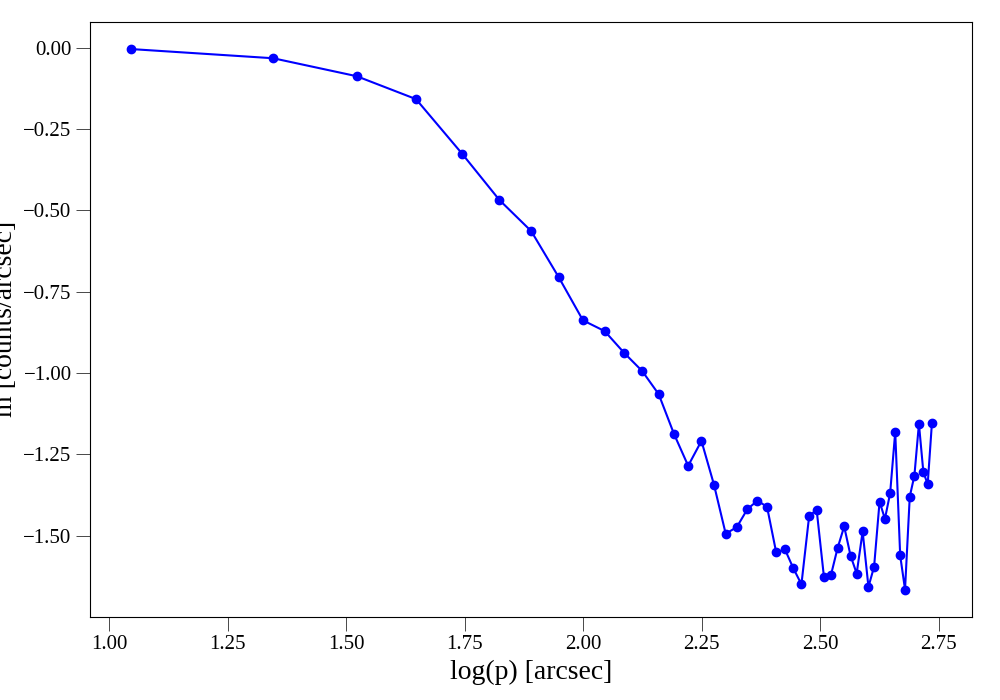
\includegraphics[width=\textwidth]{grad_counts.png}
            \captionsetup{justification=centering, font=footnotesize}
            \caption{Gradient radiálního profilu jasu povrchu komety (counts)}
            \label{fig:grad_counts}
        \end{subfigure}
        \caption{Přehled radiálních profilů a gradientů pro kometu}
        \label{fig:all_plots}
    \end{figure}
\end{document}